\chapter{Case Studies}
\label{case_studies}

This chapter uses a lot of concepts introduced in the previous ones. Its goal is to extract information from Ethereum combining 
the processing power of process mining and the execution power of the blockchain. The final objective is to find bindings 
between Ethereum transactions and extract the logic that creates them. To do this 3 case studies are presented: the first two 
are games, as usual the game industry is one of the most active in the new technology fields and for this there are a lot of 
games based on Ethereum, making this industry very interesting. Ethereum (and in general the blockchain) can be used in a lot 
of application domains: for this motivation the third case study is not about a game but instead it is about an Exchange.
Moreover this chapter has also a comparison purpose: it compares results obtained in these case studies from three algorithms: 
Split Miner, Heuristic Miner and Inductive Miner.

In Section \ref{case_studies:methodology} is defined the methodology used in the three case studies that are: 
\begin{itemize}
    \item \textbf{RotoHive} described in Section \ref{case_studies:roto};
    \item \textbf{Fomo3D} analyzed in Section \ref{case_studies:fomo};
    \item \textbf{IDEX} deepened in Section \ref{case_studies:idex};
\end{itemize}


\section{Methodology}
\label{case_studies:methodology}

As previously said the final goal of the chapter is to infer the logic which created a set of transactions resident on the 
blockchain. The blockchain technology chosen for this type of analysis is Ethereum because of one of its main components, 
the Smart Contracts. These pieces of software are public and read their code can help to better understand the behaviour of 
a system and bindings between transactions. Over that Ethereum ensures a rich environment, with a good community and many 
tools available.

\begin{figure}[!ht]
    \centering
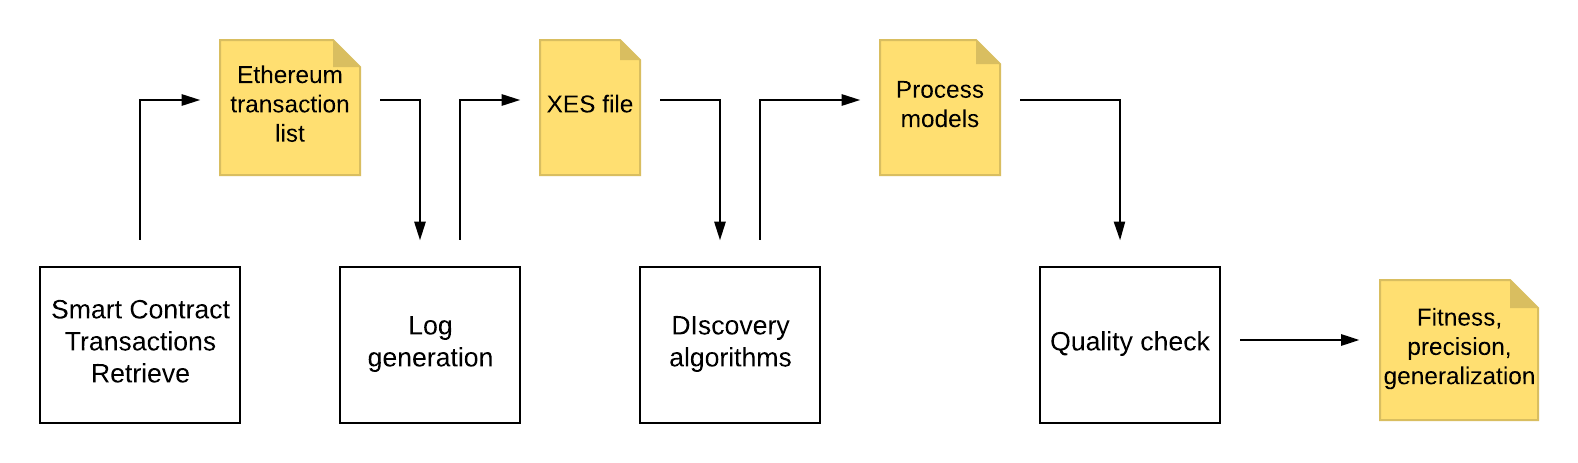
\includegraphics[width=\textwidth]{images/methodology.png}
    \caption{Methodology steps and results}
    \label{images:methodology}
\end{figure}

As shown in Figure \ref{images:methodology} the methodology applied consists of four phases:

\begin{itemize}

    \item \textbf{Smart Contract Transactions Retrieve}. The first phase of the process consists in the retrieve of a list of 
    transactions sended to a Smart Contract. This task is pretty straightforward and its done with a simple console 
    application developed in C\# that exploit an API exposed for free from Etherscan. This API returns a JSON file.

    \item \textbf{Log generation}. The second step of the process is a bit trickier than the previous. Its purpose is to 
    transform the JSON list of transactions in an event log XES file. This activity is done with an intermediate step: in a 
    first place the C\# console application transforms the JSON list in a CSV file and then this CSV is converted in XES using 
    Disco. This intermediate step is needed because there are not any libraries for XES files generation in C\#. The convertion 
    from CSV to XES in Disco is done using the transaction sender as TraceId for the final log and the method of the Smart 
    Contract invoked in that transaction (the field Input Data of the transaction) as Task. This means that in the XES log 
    generated there is one trace for each user that invoked the Smart Contract and inside each trace there is an event/task for 
    each transaction sended from that user.
    The choice of creating traces in the log by grouping transitions by sender ignores the time variable. This can bring to a 
    lost of quality of the resulting log but it is a good compromise between quality and simplicity.

    \item \textbf{Analysis}. The analysis activity start with the selection of the discovery algorithms to use: the chosen set 
    of algorithms is composed from \textbf{Heuristic Miner}, \textbf{Inductive Miner} and \textbf{Split Miner}. This choice is 
    because of the nature of these algorithms: in fact they all use different approach in the discovery process (Directly 
    Follow Graph, divide-et-conquer, Pruning and filtering) so it is a good way to understand which technique fit better in the 
    blockchain environment.
    The choice of the tool is based according to the algorithms used: in fact all these algorithms are available on Apromore and 
    not in other tools (for example ProM does not have an implementation of the Split Miner); moreover Apromore is simple to use, 
    works well and do not need local installation. The analysis activity ends with the application of the choices taken: the XES 
    log is imported in Apromore and then used as input for Split, Inductive and Heuristic Miner algorithms. At the end of this 
    step a collection of BPMN models are available.
    
    \item \textbf{Quality measurement}. The last stage of the process consist in the measure of the goodness of the results 
    obtained: as explained in chapter \ref{process_mining} the quality of a discovered model in reference to the log from which 
    it was generated can be measured using Fitness, Precision and Generalization.
    Generally these values are calculated starting from a model expressed as Petri Net. This means that a tool that converts 
    BPMN to Petri Net is needed. ProM offer a plugin called ``Convert BPMN diagram to Petri net (control-flow)" that allow for 
    this convertion. Since this is a crucial step this convertion must be verified and this can be done using rules defined in 
    \cite{DBLP:journals/BPMNtoPN} and showed in Figure \ref{images:BPMNtoPN_rules}.
    Over that ProM also has a plugin for the replay of a log on a petri net (``Reply a Log on a Petri Net for Conformance 
    Analysis"): this plugin generates a set of metrics and among them there is also the ``trace fitness" that is the fitness 
    measure. The evaluation of precision and generalization is done with a third plugin (``Measure Fitness/Generalization") that 
    starts from the result of the previous one.
    
\end{itemize}

\begin{figure}[!ht]
    \centering
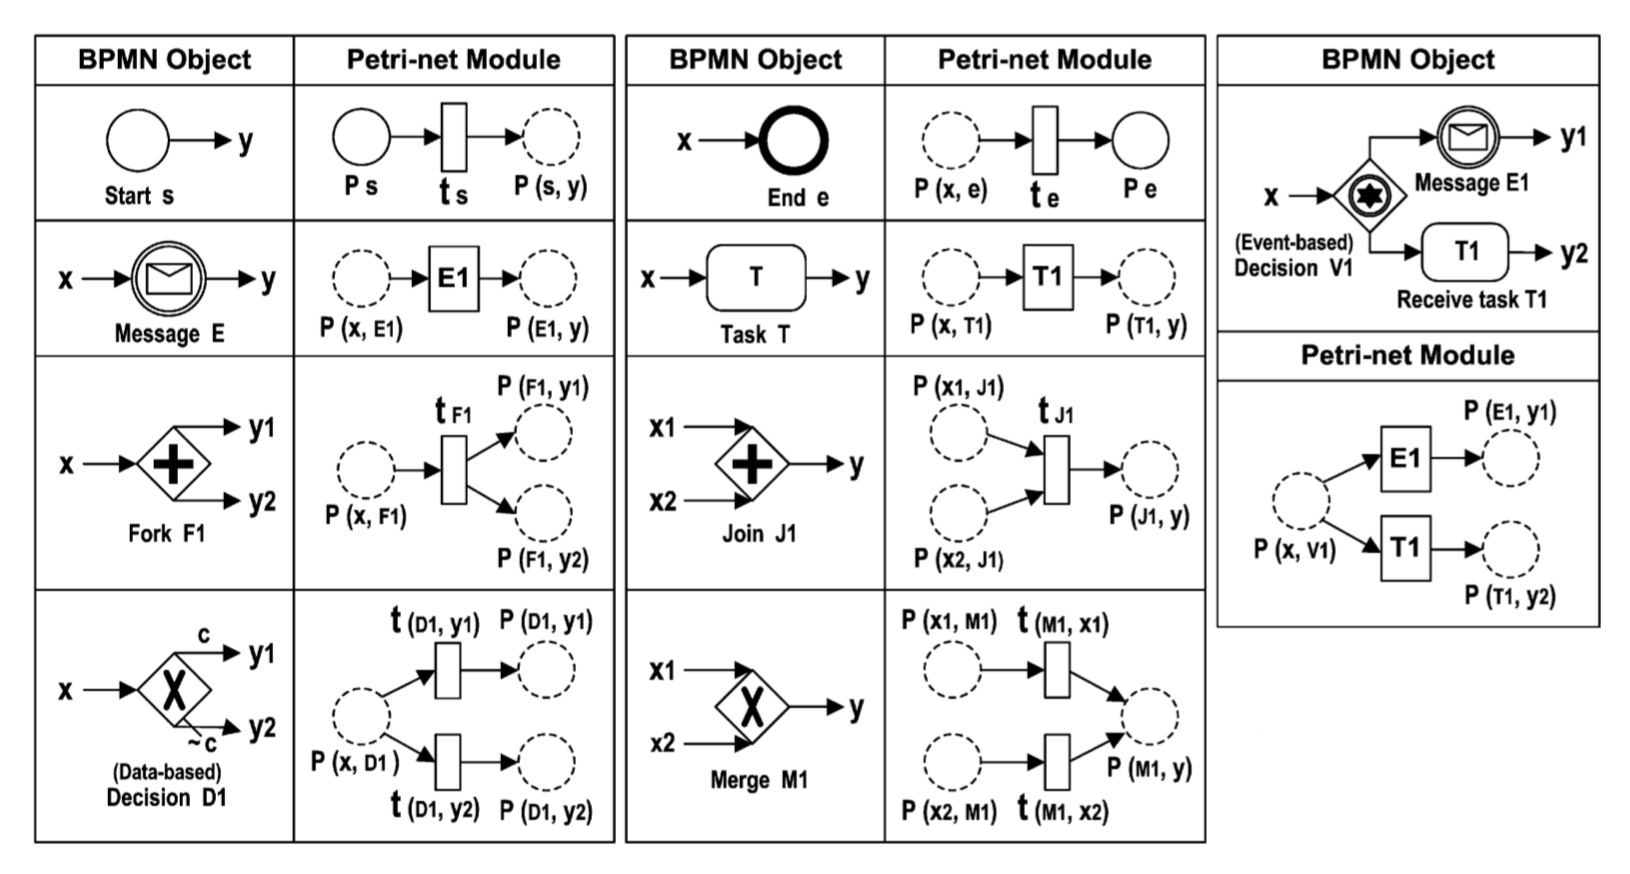
\includegraphics[width=\textwidth]{images/BPMNtoPN_rules.png}
    \caption{BPMN to Petri net conversion rules \cite{DBLP:journals/BPMNtoPN}}
    \label{images:BPMNtoPN_rules}
\end{figure}

At this point the complete process is ready to be applied to some case studies: first of all the download of the Smart Contract 
transactions, after that the building of a log starting from these transactions, then the analysis of these logs using 
different algorithms in Apromore and finally, the evaluation of the results with ProM.
In next sections these case studies are presented: the first two are games (RotoHive and Fomo3D) and the last one is an 
Exchange (IDEX).


\section{RotoHive}
\label{case_studies:roto}
RotoHive (https://www.rotohive.com) is a new type of fantasy sports site that runs weekly tournaments. It is similiar to the ``Fantacalcio", every 
Tuesday a new tournament starts and users are asked to rank NFL players by position (Quarterbacks, Running Backs, 
Wide Receivers, Tight Ends and Team Defenses) based on projected performance for the week. RotoHive user submissions are 
then rated against live player performances on Sunday and Monday night. At the end of Monday Night Football, top performing 
RotoHive users are paid for their accurate player rankings. This process then repeats on Tuesday morning when the next 
weekly tournament begins. Roto can then be staked to user submissions to win a portion of a separate weekly Ethereum prize 
pool.

The log built for RotoHive has more than 3000 events grouped in 13 different traces (this means 13 different users that played the game).
This means that even if this log considers few users the behaviour of each user with the game is quite complex with a lot of 
interactions with Ethereum (a lot of events in the log).

Figures \ref{images:roto_split}, \ref{images:roto_inductive} and \ref{images:roto_heuristic} show the resulting process models 
obtained applying, respectively, Split Miner, Inductive Miner and Heuristic Miner.

\begin{figure}[!ht]
    \centering
    \makebox[\textwidth] { 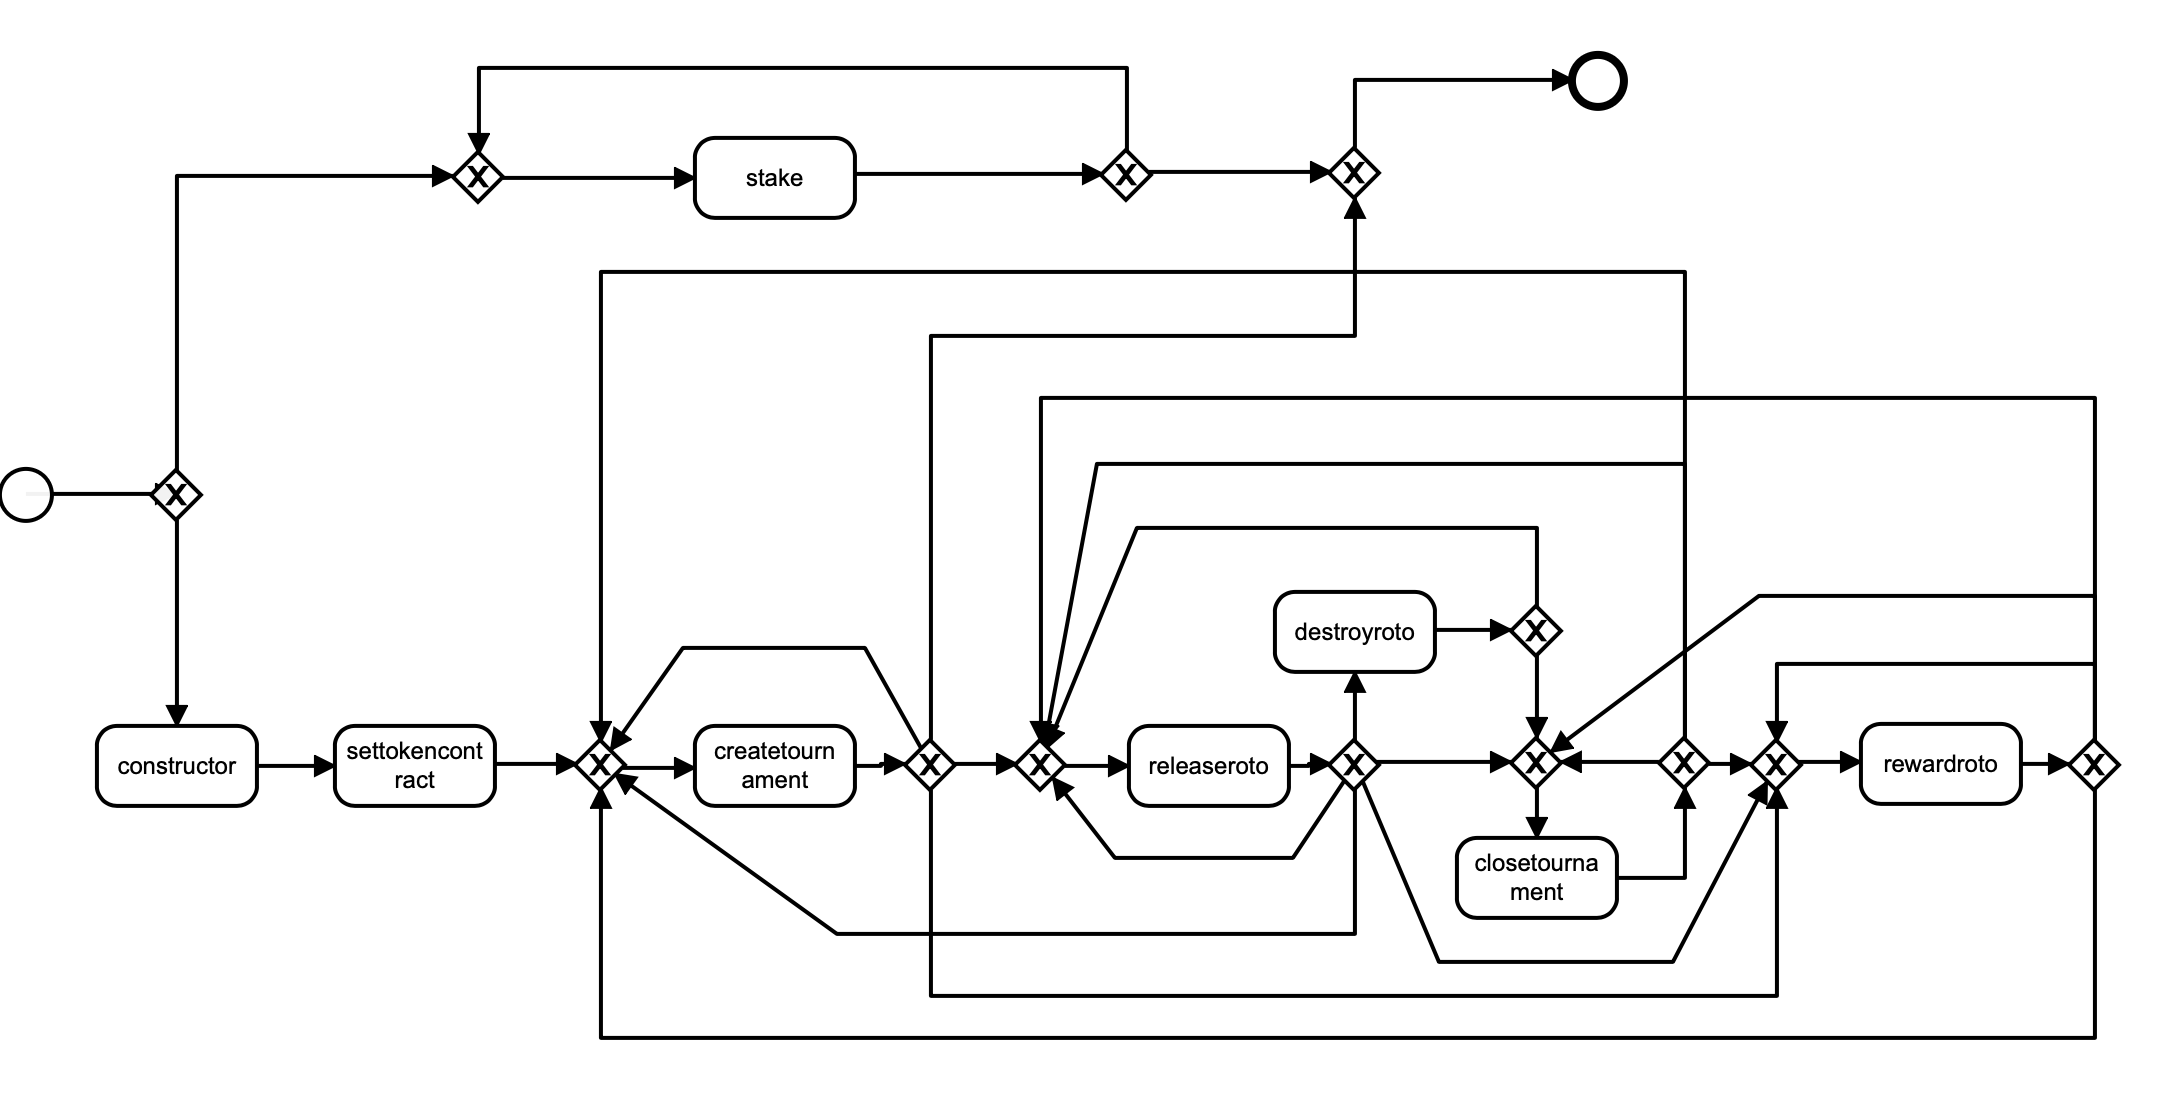
\includegraphics[width=1.2\textwidth]{images/roto_split.png} }
    \caption{RotoHive split miner}
    \label{images:roto_split}
\end{figure}

\begin{figure}[!ht]
    \centering
    \makebox[\textwidth] { 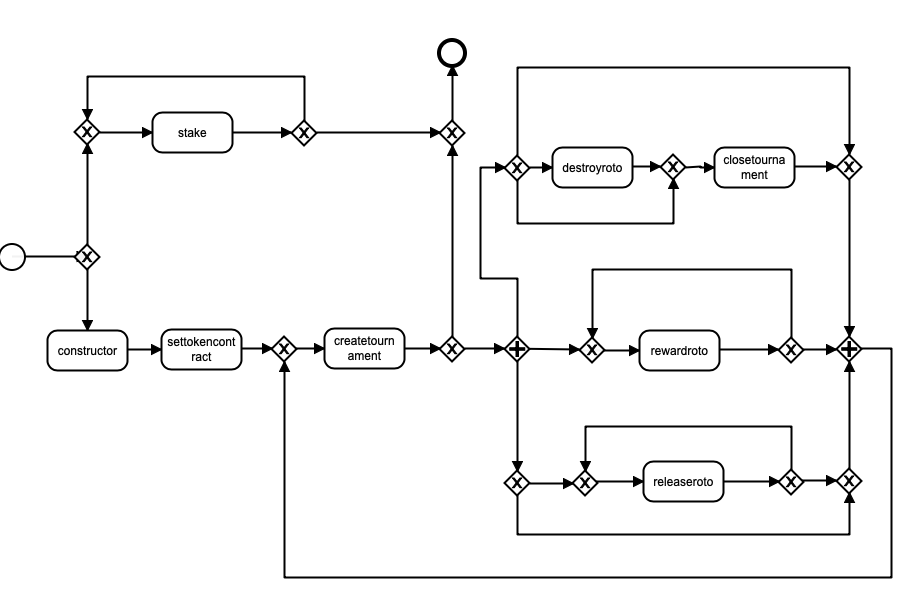
\includegraphics[width=1.2\textwidth]{images/roto_inductive.png} }
    \caption{RotoHive inductive miner}
    \label{images:roto_inductive}
\end{figure}

\begin{figure}[!ht]
    \centering
    \makebox[\textwidth] { 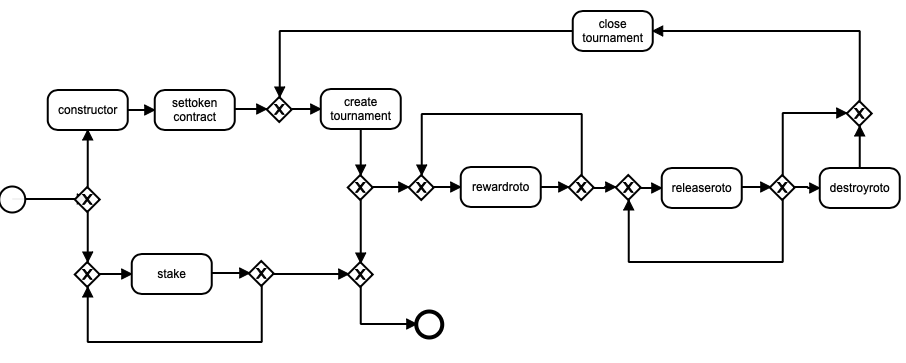
\includegraphics[width=1.2\textwidth]{images/roto_heuristic.png} }
    \caption{RotoHive heuristic miner}
    \label{images:roto_heuristic}
\end{figure}


In general in the model there is a main fork that split the process for user: a first part is for common users that can only 
stake their Roto in order to win Ether and a second part that is for the admin of the system who can create a tournament, 
distribute Roto to winners or destroy Roto for bad performances and than close the tournament in a weekly cycle.

Table \ref{tables:roto} shows the results of the qualitative measures on the models:

\begin{center}
    \label{tables:roto}
    \begin{tabular}{ | l | c | c | c | c |}
        \hline
        \textbf{Algorithm} & \textbf{BPMN to PN} & \textbf{Fitness} & \textbf{Precision} & \textbf{Generalization} \\ 
        \hline
        Split Miner & Ok & 1 & 0.20453 & 0.99892 \\ 
        \hline
        Inductive Miner & Ok & 0.99995 & 0.60294 & 0.99496 \\
        \hline
        Heuristic Miner & Ok & 0.99940 & 0.49889 & 0.99889 \\
        \hline
    \end{tabular}
\end{center}

We can see that Fitness and Generalization values a pretty high in each algorithm while Precision is more variable and in 
general values are smaller. The evaluation of the conversion between BPMN and Petri Net is done using rules described 
previously. In general all the three models represents quite well the application domain but those discovered with Split Miner 
and Inductive Miner are too confusing. Simplicity is an important aspect and for this motivation the Heuristic Miner is the 
algorithm that performed better in this case study.


\section{Fomo3D}
\label{case_studies:fomo}

Here's Fomo3D (https://exitscam.me/play) in a nutshell:

\begin{itemize}
    \item This is a lottery game in which the last person to buy a key at the end of a round wins the jackpot!
    \item During a round, people can purchase 1 or more keys which resets the timer marking them as the current leader. With each key purchase during the round, the key price increases slightly.
    \item Players receive a stream of passive income from the game as keys are bought during the round.
    \item When the timer reaches zero, last person to buy a key wins! (F3D players/P3D holders get a piece too!)    
\end{itemize}

With a few cool game mechanics:

\begin{itemize}
    \item There are two different game modes with distinct rules and round durations: Long and Soon.
    \item Players can select from one of four teams which determine certain rules in the round.
    \item P3D holders receive dividends on each key purchase and at the end of the round.
    \item Players can buy a vanity URL and/or refer your friends to the game for extra rewards.
    \item Buying keys offers you a \% chance to receive an ``airdrop" winning ETH from a growing side-jackpot!
\end{itemize}

At the end of the round, the ETH in the jackpot is divvied up: the winner receives half of the jackpot, with the rest split 
between all F3D players as well as to P3D holders. The specific way the ETH is divided between the F3D participants 
and the P3D holders depends on which team the winner was representing. 

The resulting log in this case contains more traces than RotoHive (so more users for the game), about 40, but with less 
interactions with the smart contract in fact on average there are only three events per each trace.

In Figures \ref{images:fomo_split}, \ref{images:fomo_inductive} and \ref{images:fomo_heuristic} the resulting models 
obtained after the analysis based on, respectively, Split Miner, Inductive Miner and Heuristic Miner.

\begin{figure}[!ht]
    \centering
    \makebox[\textwidth] { 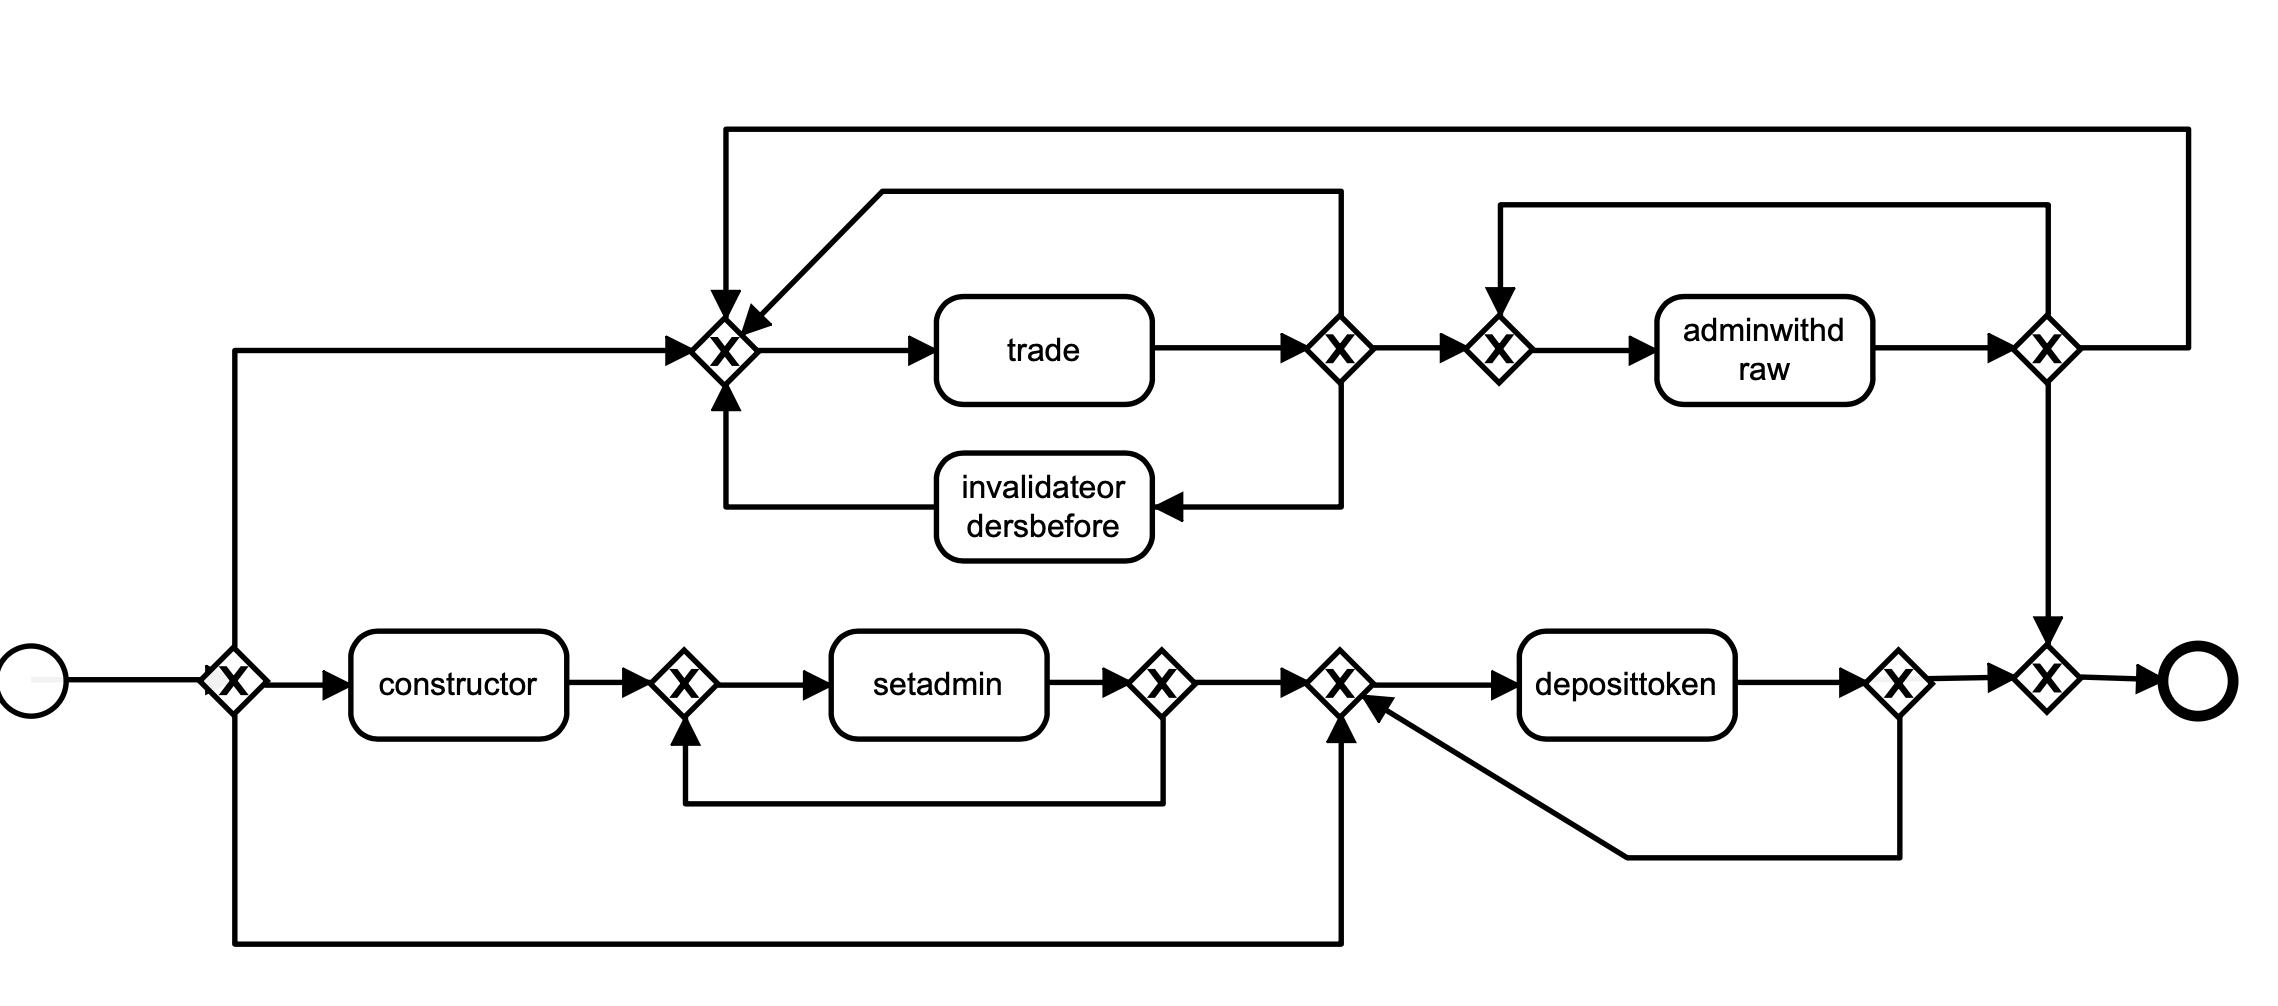
\includegraphics[width=1.2\textwidth]{images/fomo_split.png} }
    \caption{Fomo3D split miner}
    \label{images:fomo_split}
\end{figure}

\begin{figure}[!ht]
    \centering
    \makebox[\textwidth] { 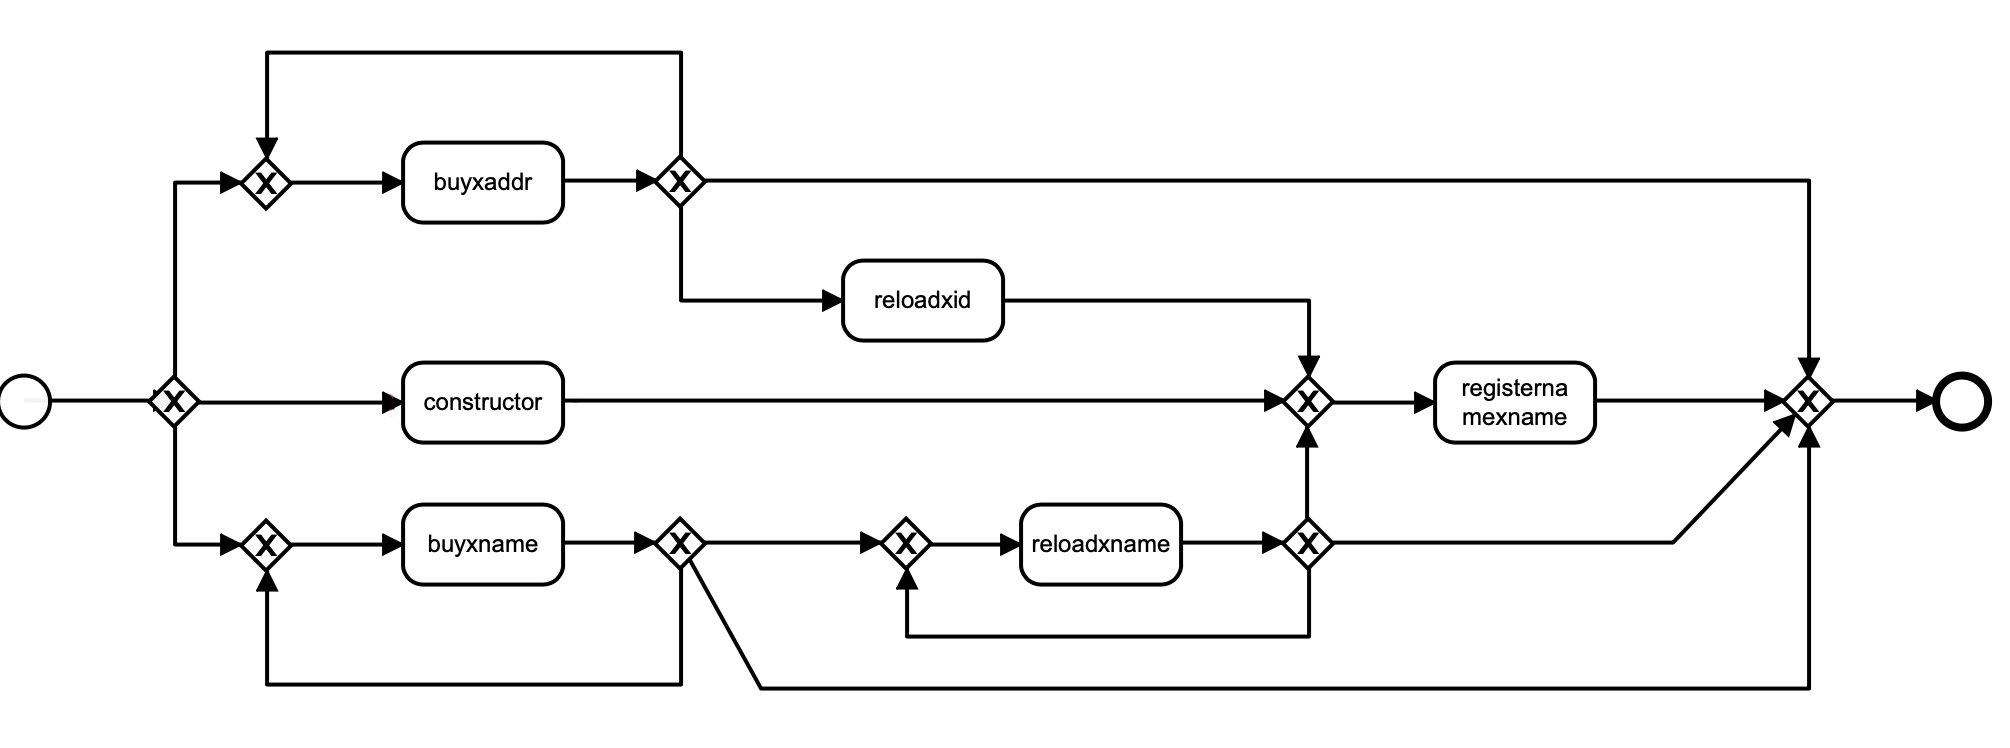
\includegraphics[width=1.2\textwidth]{images/fomo_inductive.png} }
    \caption{Fomo3D inductive miner}
    \label{images:fomo_inductive}
\end{figure}

\begin{figure}[!ht]
    \centering
    \makebox[\textwidth] { 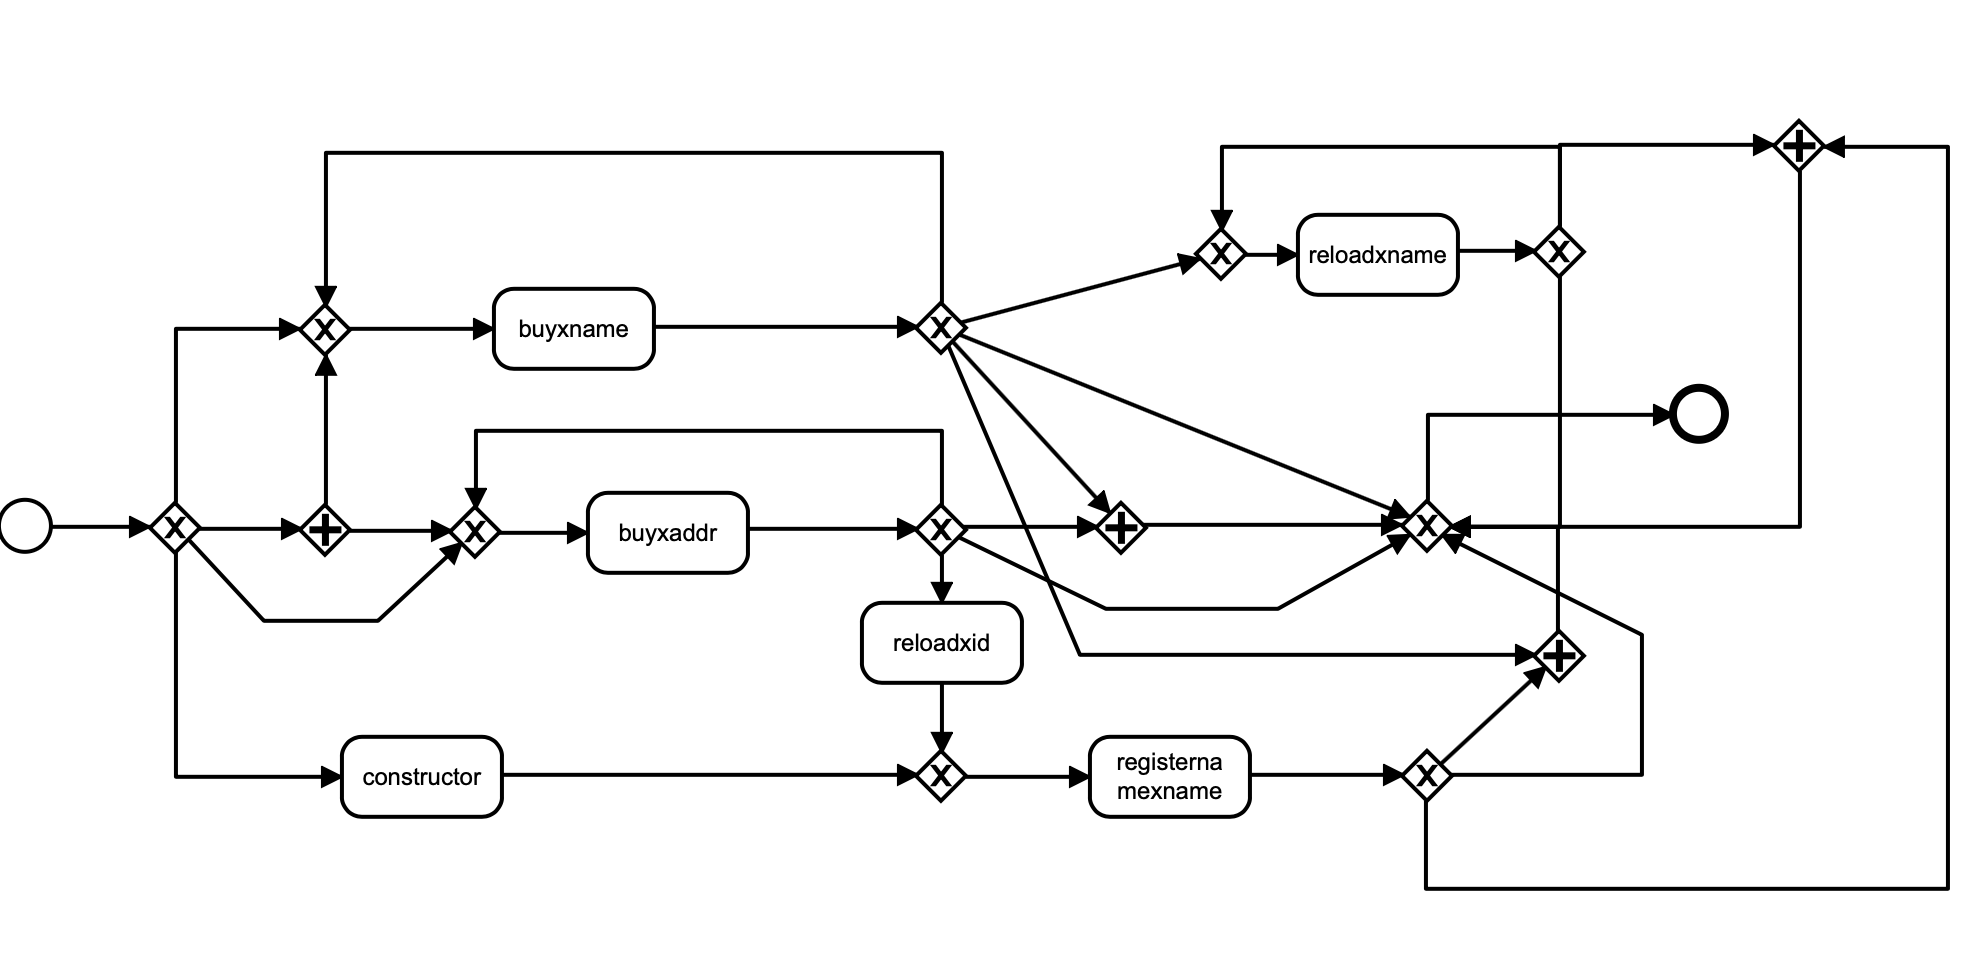
\includegraphics[width=1.2\textwidth]{images/fomo_heuristic.png} }
    \caption{Fomo3D heuristic miner}
    \label{images:fomo_heuristic}
\end{figure}

Both tasks ``buy*" and ``reload*" has a similar behaviour: they spends ETH to purchase keys in order to win the jackpot but with a 
small difference: ``buy*" use ETH from user wallet instead ``reload*" uses your unwithdrawn earnings. This is explained in a 
comment of the smart contract available on Ethereum.

In Table \ref{tables:fomo} the quality values measured:

\begin{center}
    \label{tables:fomo}
    \begin{tabular}{ | l | c | c | c | c |}
        \hline
        \textbf{Algorithm} & \textbf{BPMN to PN} & \textbf{Fitness} & \textbf{Precision} & \textbf{Generalization} \\ 
        \hline
        Split Miner & Ok & 0.97357 & 0.47947 & 0.96836 \\ 
        \hline
        Inductive Miner & Ok & 0.97357 & 0.47947 & 0.96836 \\
        \hline
        Heuristic Miner & Ok & 0.98710 & 0.48634 & 0.87593 \\
        \hline
    \end{tabular}
\end{center}

Even in this case fitness and generalization values are pretty high while precision is smaller even if more stable than the 
previous example. From the generalization point of view only heuristic miner has a bit smaller value. For Fomo3D both Split 
Miner and Inductive Miner discovered the same model and obviously also the quality measures are the same. Heuristic Miner 
this time inferred also the dirtier model. So in this case Split Miner and Inductive Miner perform better than Heuristic.


\section{IDEX}
\label{case_studies:idex}

Exchanges are applications that allows the user to deposit, withdraw or exchange cryptocurrencies: one of the most famous 
and used exchange running on Ethereum is IDEX (https://idex.market/eth/). IDEX is the first Ethereum based decentralized smart contract exchange to 
support real-time trading and high transaction throughput. IDEX is the most advanced Ethereum DEX, supporting limit and market 
orders, gas-free cancels, and the ability to fill many trades at once. IDEX allows users to trade all ERC20 tokens: ERC20 is 
an Ethereum standard that define the base behaviour of a token. On top of the standard, custom features can be added.
IDEX allow to buy/sell tokens using two approaches: 

\begin{itemize}
    \item \textbf{Limit order}, where the user define the amount of tokens to buy/sell, the token, and a limit: when the 
        value of the token reaches (increasing or decreasing) the limit defined the transaction will be commited to Ethereum. 
        Until that moment the transaction is in a pending state.
    \item \textbf{Market order}, in this case instead the transaction is commited immediatly using the current market value 
        of the token.
\end{itemize}

In this case the built log contains more than 2000 events grouped in 14 traces. Even in this case every user has a lot of interaction 
with the smart contract.

Figure \ref{images:idex_split} shows the model obtained applying the Split Miner algorithm, in Figure \ref{images:idex_inductive} 
is depicted the model inferred throug Inductive Miner and, finally Figure \ref{images:idex_heuristic} shows the result of the 
Heuristic Miner algorithm. 

\begin{figure}[!ht]
    \centering
    \makebox[\textwidth] { 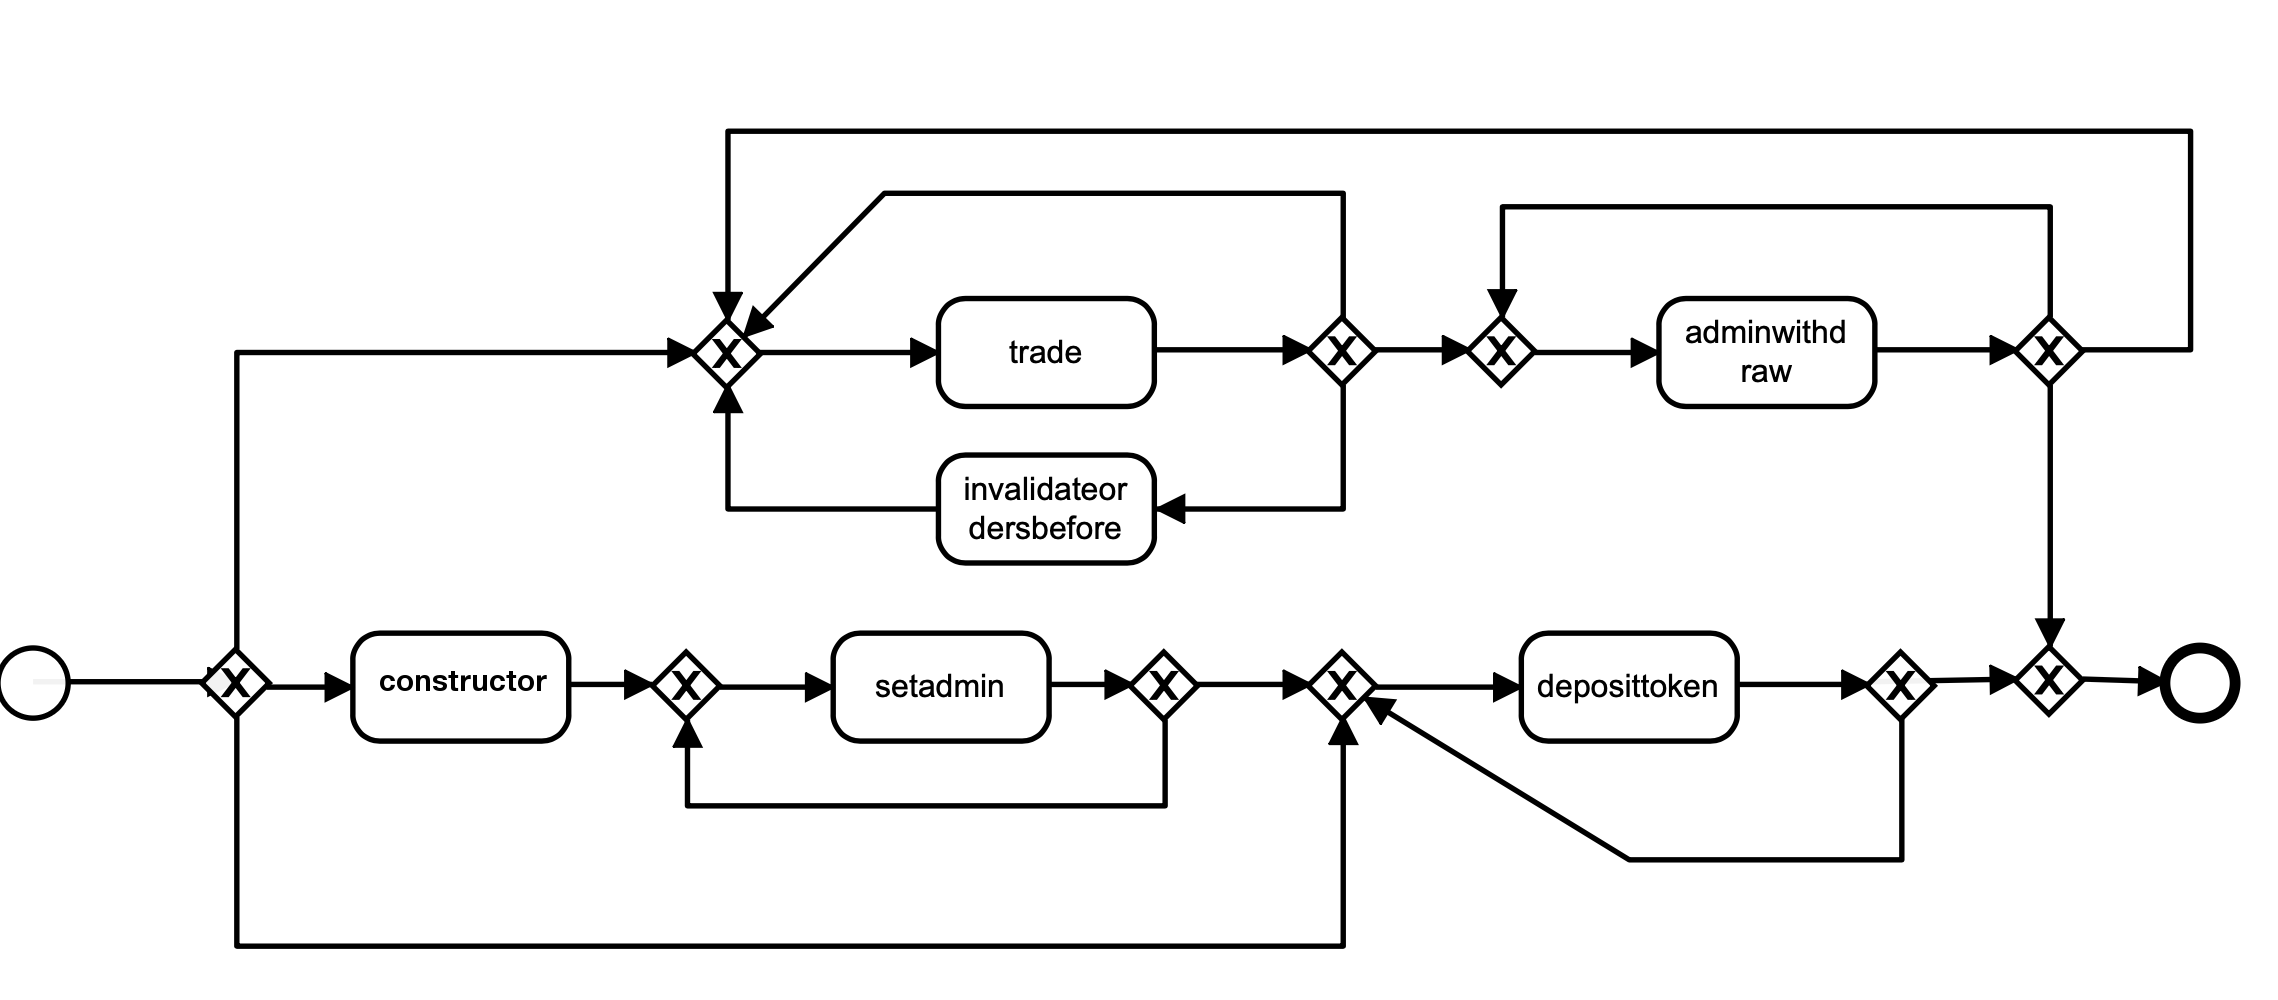
\includegraphics[width=1.2\textwidth]{images/idex_split.png} }
    \caption{IDEX split miner}
    \label{images:idex_split}
\end{figure}

\begin{figure}[!ht]
    \centering
    \makebox[\textwidth] { 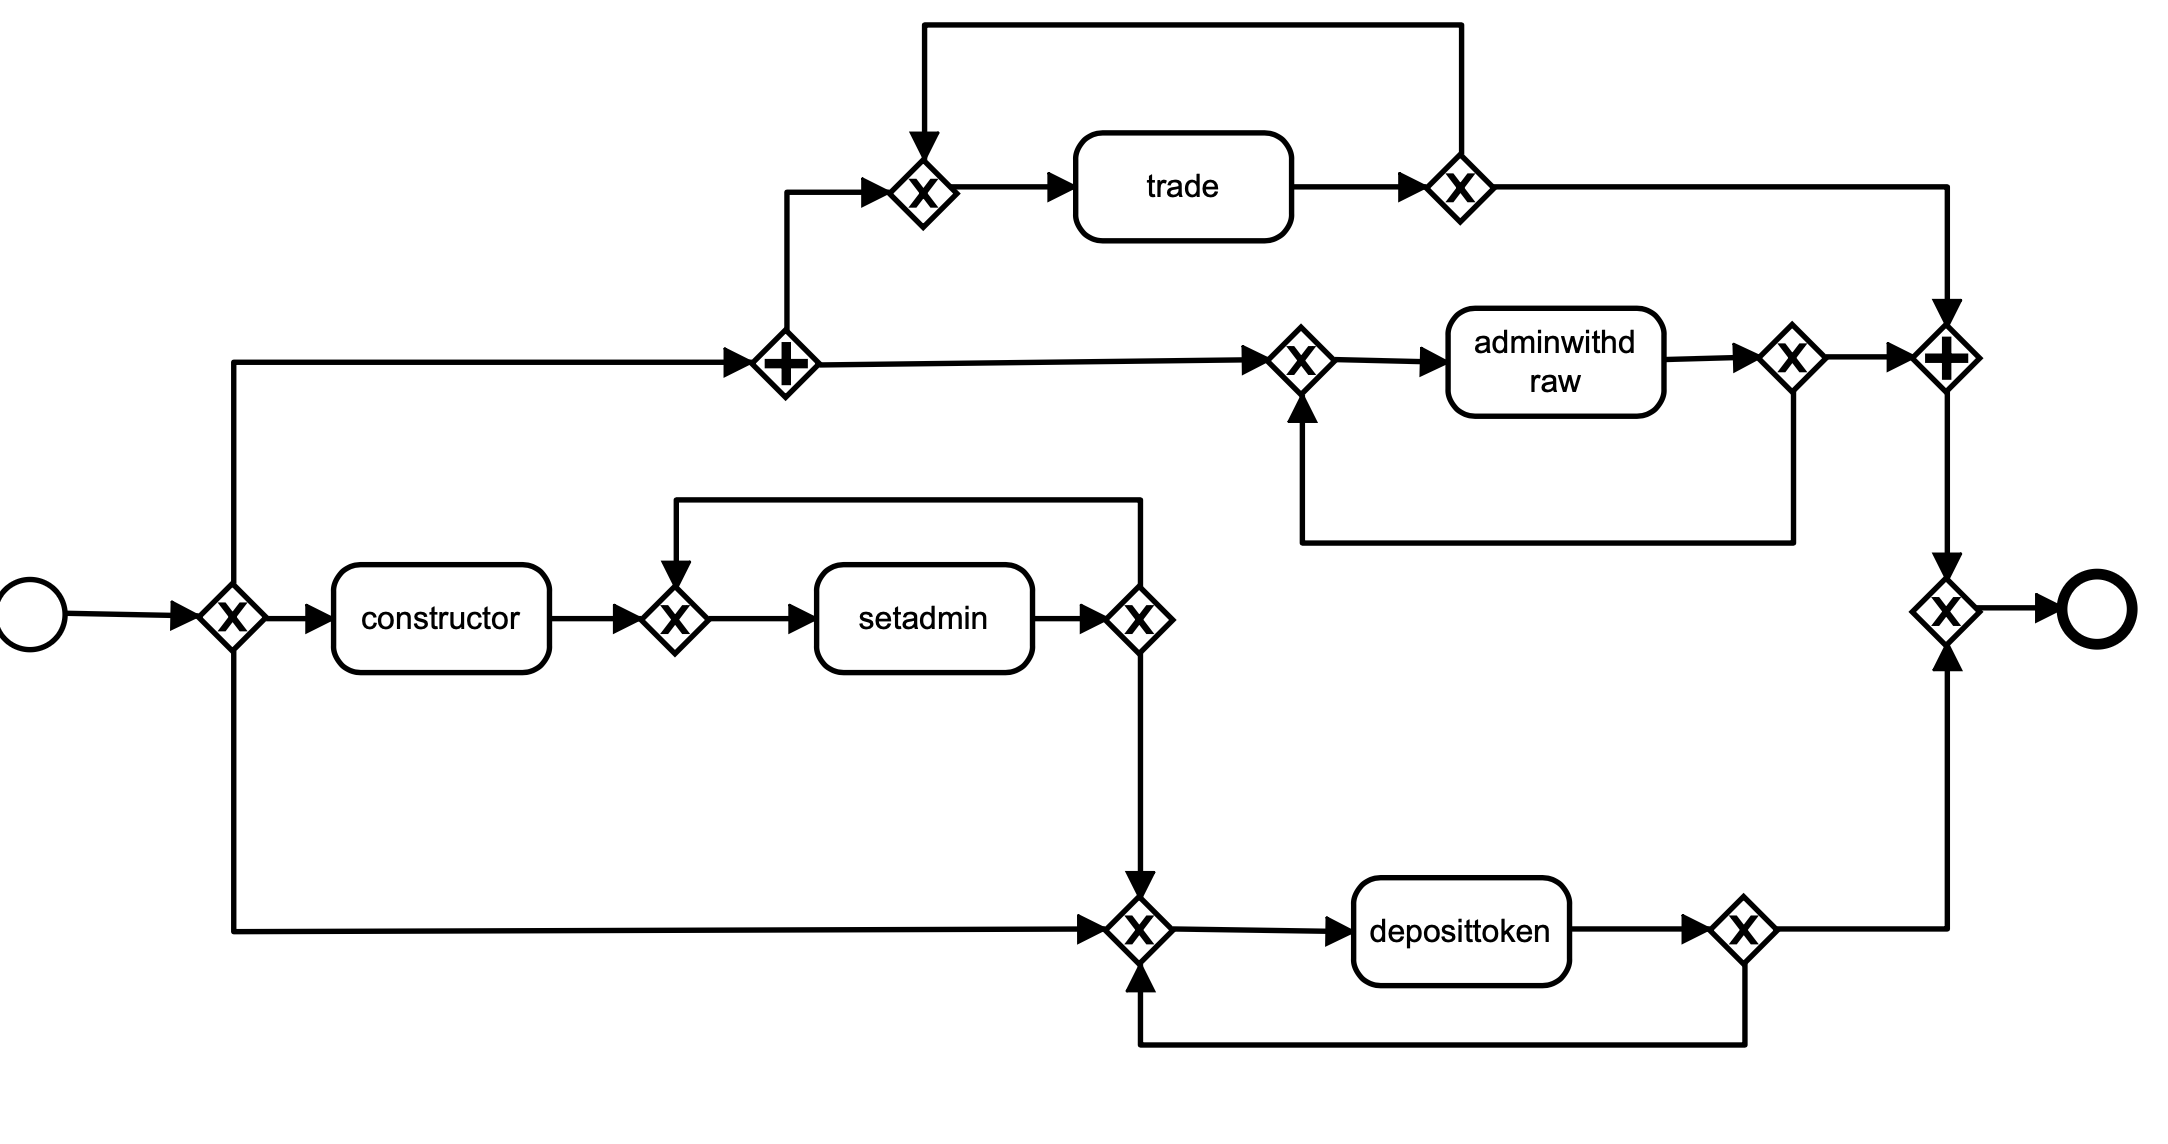
\includegraphics[width=1.2\textwidth]{images/idex_inductive.png} }
    \caption{IDEX inductive miner}
    \label{images:idex_inductive}
\end{figure}

\begin{figure}[!ht]
    \centering
    \makebox[\textwidth] { 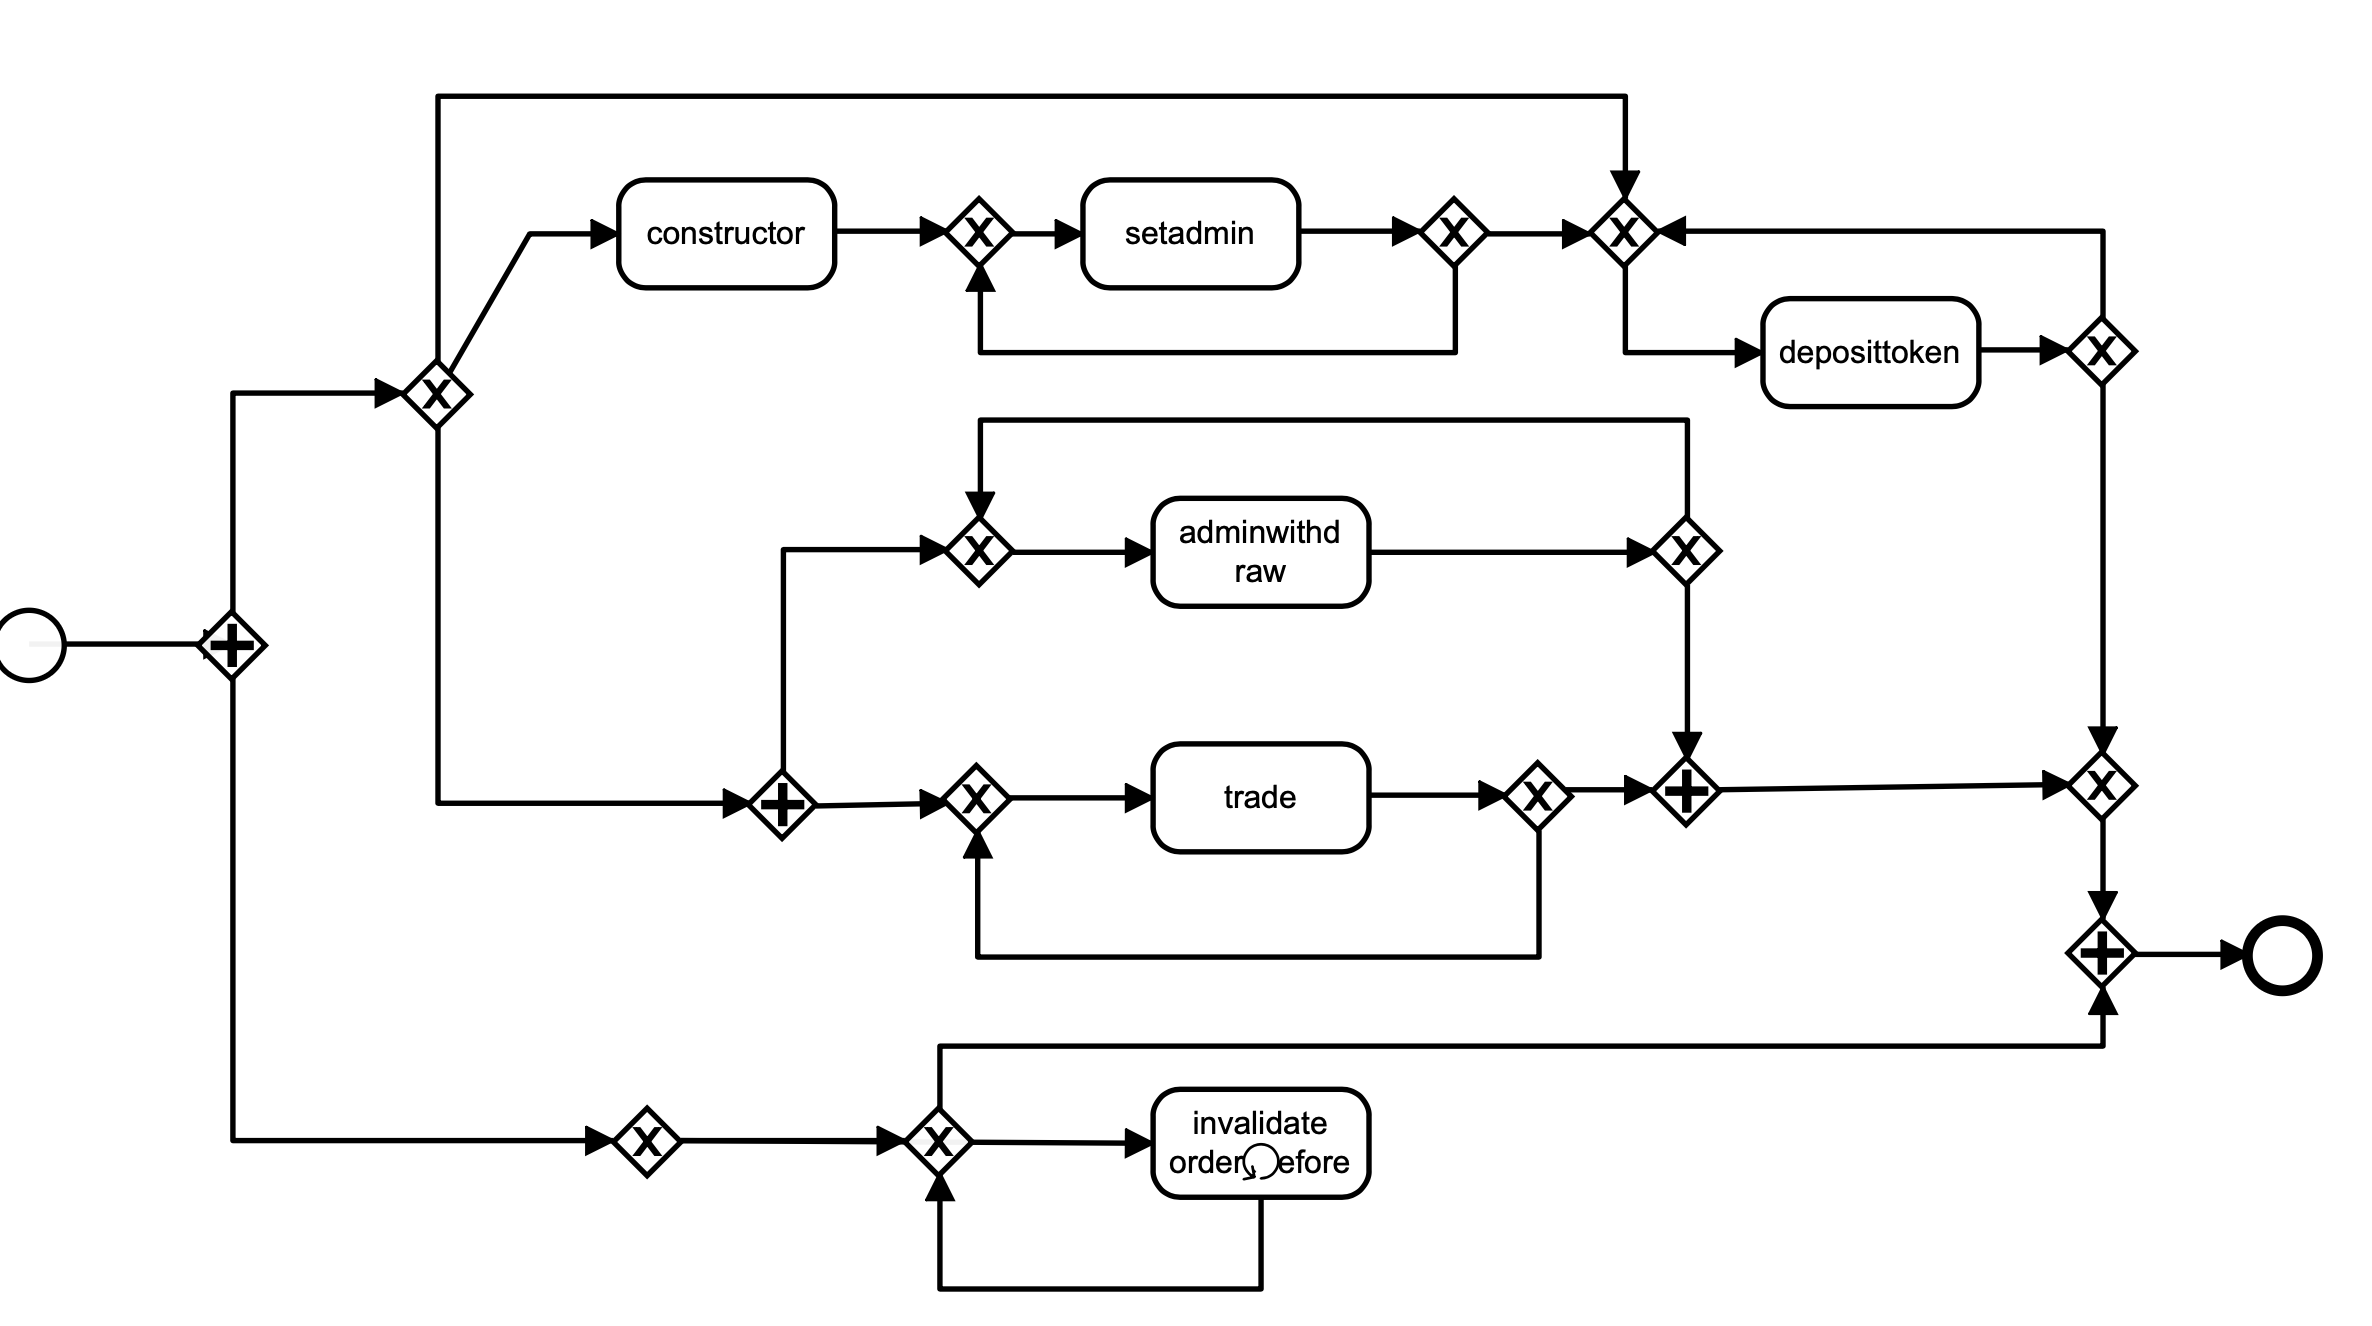
\includegraphics[width=1.2\textwidth]{images/idex_heuristic.png} }
    \caption{IDEX heuristic miner}
    \label{images:idex_heuristic}
\end{figure}

Table \ref{table:idex_results} shows the quality values measured:

\begin{center}
    \begin{tabular}{ | l | c | c | c | c |}
        \hline
        \textbf{Algorithm} & \textbf{BPMN to PN} & \textbf{Fitness} & \textbf{Precision} & \textbf{Generalization} \\ 
        \hline
        Split Miner & Ok & 0.99573 & 0.22884 & 0.99914 \\ 
        \hline
        Inductive Miner & Ok & 0.99971 & 0.48298 & 0.99968 \\
        \hline
        Heuristic Miner & Ok & 1 & 0.32516 & 0.99882 \\
        \hline
    \end{tabular}
    \label{table:idex_results}
\end{center}

As in the previous cases Fitness and Generalization are stable and high, instead Precision is less stable and not so high.
This time analysing the models the Inductive Miner skipped a task (it was filtered out) but despite this it performed 
better than the others in the quality measures expecially for the Precision. From the point of view of models readability all 
the three algorithms performed well in this case study.


\section{Lessons learned}
The used approach has allowed to obtain good results with sound models discovered and pretty good quality parameters 
measured. Even if the process is a bit articulated and mechanical the used tools were simple to use, reliable and 
they work well together.
In the construction phase of the log the choice to group the transitions for smart contracts has been a winning one 
because it has highlighted a link between the different transitions. One aspect that could be improved during the building of 
the log is to take in consideration the time variable during the grouping of the activities in traces: an idea can be to do 
some clustering defining the time interval of a trace.

The analysis of how and how many transitions use a smart contract results in deducing the logic with which these transitions 
were generated, ie the logic of the DAPPs. This analysis can be seen as a kind of reverse engeenering. 

The three different algorithms used have obtained very similar results and in every case study a different algorithm performed 
better than the others. In general these observations let think that the measure of how well an algorithm fits a specific 
application domain depends from the business logic of this domain regardless the fact that it uses the Blockchain.

Potentially the methodology used in this chapter, adequately refined, could also be used to understand how a user interacts with 
a system and compares different behaviors. Going even further in this direction we could understand the tastes and 
characteristics of certain users by analyzing how they interacted on different systems.